\chapter{¿Por qué sube y baja la bolsa de valores?}

\section{Introducción}

La bolsa de valores es uno de los mercados financieros más importantes y a menudo genera una gran cantidad de incertidumbre y especulación. Los precios de las acciones y otros activos financieros suben y bajan debido a múltiples factores \parencite{@5287-FREDERIC2018,@5286-ZVI2013}. En este artículo, analizaremos algunos de los principales factores que afectan el movimiento de la bolsa y presentaremos una explicación económica de estos movimientos. Utilizaremos fórmulas económicas y un diagrama para ilustrar los conceptos clave.

\section{Factores que afectan la bolsa de valores}

Los precios en la bolsa de valores están influenciados por factores tanto macroeconómicos como microeconómicos. Los más importantes incluyen:

\begin{itemize}
\item \textbf{Noticias económicas}: informes de inflación, tasas de interés y crecimiento económico afectan las expectativas de los inversionistas.
\item \textbf{Política monetaria}: las decisiones del banco central sobre las tasas de interés influyen directamente en el costo de capital y las expectativas de los rendimientos.
\item \textbf{Resultados empresariales}: los ingresos y utilidades reportados por las empresas influyen en la percepción del valor de sus acciones.
\end{itemize}

\section{Modelo del precio de las acciones}

El valor de una acción puede ser modelado utilizando el enfoque de los flujos de caja descontados (\textit{Discounted Cash Flow, DCF}). El precio de una acción $P_0$ puede expresarse como la suma de los dividendos futuros esperados $D_t$, descontados a una tasa de descuento $r$, que representa el riesgo del activo:

\begin{equation}
P_0 = \sum_{t=1}^{\infty} \frac{D_t}{(1 + r)^t}
\end{equation}

Este modelo sugiere que los precios de las acciones subirán si los dividendos futuros esperados aumentan o si la tasa de descuento disminuye. Por el contrario, los precios bajarán si las expectativas de dividendos disminuyen o si la tasa de descuento aumenta.

\section{Oferta y demanda en el mercado}

El precio de una acción está determinado por la oferta y la demanda en el mercado de valores. Si la demanda de una acción supera la oferta, su precio subirá, y si la oferta supera la demanda, el precio caerá. Esto se puede modelar matemáticamente mediante una función de demanda:

\begin{equation}
Q_d = f(P, I, r)
\end{equation}

Donde:
\begin{itemize}
\item $Q_d$ es la cantidad demandada de acciones.
\item $P$ es el precio de la acción.
\item $I$ es el ingreso de los inversionistas.
\item $r$ es la tasa de interés.
\end{itemize}

De manera similar, la cantidad ofertada de acciones $Q_s$ está influenciada por factores como la liquidez y el número de acciones disponibles.

\section{Diagrama de la dinámica del mercado}

A continuación se presenta un diagrama simplificado utilizando TikZ, que muestra cómo interactúan la oferta y la demanda en el mercado de valores:

\begin{figure}[h!]
\centering
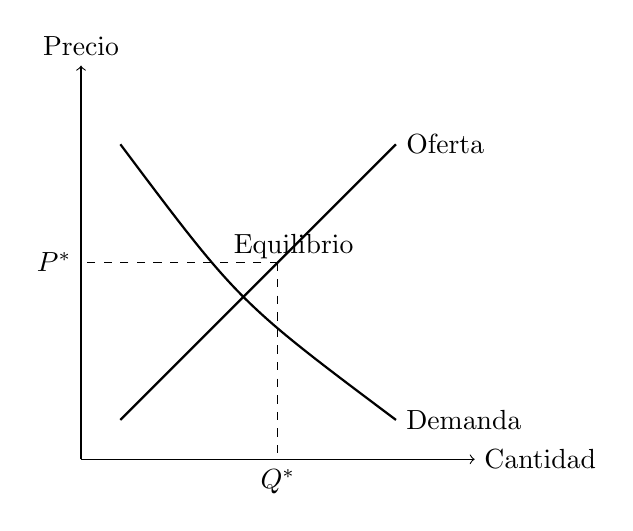
\begin{tikzpicture}
% Ejes
\draw[->] (0,0) -- (5,0) node[right] {Cantidad};
\draw[->] (0,0) -- (0,5) node[above] {Precio};

% Curva de demanda
\draw[thick] (0.5,4) .. controls (2,2) .. (4,0.5) node[right] {Demanda};

% Curva de oferta
\draw[thick] (0.5,0.5) .. controls (2,2) .. (4,4) node[right] {Oferta};

% Punto de equilibrio
\draw[dashed] (2.5,2.5) -- (2.5,0) node[below] {$Q^*$};
\draw[dashed] (2.5,2.5) -- (0,2.5) node[left] {$P^*$};

% Etiqueta de equilibrio
\node at (2.7,2.7) {Equilibrio};
\end{tikzpicture}
\caption{Interacción de la oferta y la demanda en el mercado de valores.}
\end{figure}

En este gráfico, el punto de equilibrio $(Q^*, P^*)$ representa el precio y la cantidad donde la oferta y la demanda se igualan. Si ocurre un cambio en alguno de los factores determinantes de la demanda o la oferta, el punto de equilibrio se desplazará, afectando el precio de las acciones.

\section{Factores adicionales}

Además de la oferta y la demanda, otros factores juegan un papel importante en los movimientos de la bolsa:

\subsection{Política monetaria y fiscal}
Las tasas de interés son un factor crucial en la valoración de activos financieros. Según el modelo CAPM (Capital Asset Pricing Model), el retorno esperado de un activo financiero $E(R_i)$ se calcula como:

\begin{equation}
E(R_i) = R_f + \beta_i (E(R_m) - R_f)
\end{equation}

Donde:
\begin{itemize}
\item $R_f$ es la tasa libre de riesgo.
\item $\beta_i$ es la sensibilidad del activo $i$ respecto al mercado.
\item $E(R_m)$ es el retorno esperado del mercado.
\end{itemize}

Este modelo indica que si la tasa libre de riesgo \(R_f\) aumenta, el retorno esperado de las acciones también aumentará, lo que puede provocar una caída en los precios actuales de las acciones debido a que los inversionistas exigen mayores rendimientos.

\subsection{Expectativas del mercado}

Las expectativas de los inversionistas sobre el futuro son otro factor clave que afecta el precio de las acciones. Los cambios en las expectativas pueden deberse a informes económicos, cambios en la política gubernamental o eventos inesperados como crisis económicas o avances tecnológicos.

\section{Conclusión}

El precio de las acciones en la bolsa de valores está determinado por una compleja interacción de factores económicos y psicológicos. Las fórmulas de valoración financiera, como el modelo de flujos de caja descontados y el CAPM, nos brindan herramientas para entender cómo la información disponible y las expectativas futuras influyen en los movimientos del mercado. Sin embargo, dado que los mercados financieros también están sujetos a la especulación y al comportamiento de los inversionistas, siempre existe un grado de incertidumbre asociado a los movimientos de la bolsa.
